The correctness of the leaf-level components introduced by CASE
transformations resolves to the question of whether such a component
meets its \agree{} contract. This obligation is addressed by
\emph{formal synthesis}: given a sufficiently detailed formal
specification of component behavior, the \splat{} tool generates code
from it and also generates proofs showing that the generated code is
correctly compiled and meets its specification.

The formal languages that filters, gates, and monitors are generated
from include regular expressions, contiguity types
\cite{contiguity-types}, and Lustre \cite{lustre}. For each of these
languages, we have infrastructure (see Figure \ref{fig:synthesis})
that (a) translates formal specifications to code and (b) proves the
correctness of the translation using the HOL4 system
\cite{hol4:overview}. The generated code is \emph{CakeML}, a dialect
of Standard ML \cite{SML97} possessing a fully verified compiler
\cite{cakeml}.

\begin{figure}[h]
\begin{center}
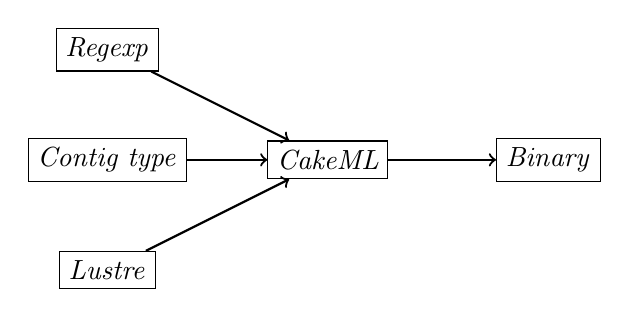
\begin{tikzpicture}[scale = 0.7]
\node (A) at (0,2) [shape=rectangle,draw]{\textit{Regexp}};
\node (B) at (0,0) [shape=rectangle,draw]{\textit{Contig type}};
\node (C) at (0,-2) [shape=rectangle,draw]{\textit{Lustre}};
\node (D) at (4,0) [shape=rectangle,draw]{\textit{CakeML}};
\node (E) at (8,0) [shape=rectangle,draw]{\textit{Binary}};
\draw [->,thick] (A) to (D);
\draw [->,thick] (B) to (D);
\draw [->,thick] (C) to (D);
\draw [->,thick] (D) to (E);
\end{tikzpicture}
\end{center}
\caption{\splat{} Verified Synthesis Path.\label{fig:synthesis}}
\end{figure}

Regular expressions and contiguity types are formalisms well-suited
for expressing classes of constraints on the data passed in
messages. Thus they provide a useful basis for expressing
filters. Regular expressions compile to efficient finite state
automata, generating a correctness proof along the way
\cite{case-verified-filter}.  We have also synthesized regular
expressions to hardware using this proof-producing
technique \cite{formal-filter-synth-langsec}.
Contiguity types can capture more complex
data formats, including variable-length arrays and union structures;
this level of expressiveness was needed to handle the messages of
UxAS. We deploy a verified contiguity-type based parser generator
\cite{contiguity-types} to decode and check the wellformedness of
such serialized data.

Gates and monitors can require arbitrarily complex computations for
their work; hence we also support code generation from Lustre. We have
formalized the semantics of Lustre and are using it as the basis for a
formal translation to CakeML.

Since code generated from \splat{} is deployed as a scheduled thread
in a real-time environment, there are two aspects to consider: (1)
correctness of a `one shot` thread execution (discussed above), and
(2) correctness of the perpetual re-execution of the thread. How to
model the latter and prove relevant properties is discussed in
\cite{johannes:repeat}.
